\documentclass{article}
\usepackage[french]{babel}
\usepackage[T1]{fontenc}
\usepackage[utf8]{inputenc}
\usepackage{graphicx}
\usepackage{eurosym}
\usepackage {times}
\usepackage{fancyhdr}
\usepackage{bm}
\usepackage{listings}
\title{Projet CamlT'OCR par SMK \~Cahier des charges}
\pagestyle{fancyplain} \lhead{\textit{Projet CamelT'OCR}} \rhead{\textit{SMK}}
\date{24-10-2014}
\author{
    Timothe \textit{Tim-Tim} Bureau-Godart(bureau\_t) \and
        Leopold \textit{Meta} Szabatura (szabat\_l) \and
        Louis \textit{Zab} Forget (forget\_l) \and
        Maxime \textit{Kylox} Gaudron (gaudro\_m)
        1      }


\begin{document}
\begin{center}
\maketitle
\end{center}
\newpage
\tableofcontents
\newpage
\section{Introduction}
\addcontentsline{toc}{section}{Introduction}
Dans le cadre de notre specialisation en informatique a l'EPITA, nous avons eu comme projet smestrielle la realisation d'un ocr ( Optical Character Recognition). Ce projet ce deroule sur 4 mois en Ocaml, un langage develloper par l'INRIA. Nous presentons donc dans ce rapport l'etat d'avancement du projet a la vielle de la premiere soutenance. Ce projet a ete realise par quattre membre fidele et devoue a la bonne cause celle de notre ocr ! 
\subsection{presentation des membres}
\subsubsection{Louis "\textit{Zab}" Forget}
J'ai toujours etais tres curieux, au point de partir souvent dans tous les sens. J'ai toujours voulu savoir comment marchent les pages webs. C'est dans cette optique que j'ai appris a faire du HTML et CSS en troisieme. J'ai ensuite voulu savoir comment marchent les jeux videos, puis divers programmes. Il y a quelques jours je me suis demandais commemt marchent les gps qui indiquent la densite du traffic.
\subsubsection{Timothe "\textit{Tim-Tim}" Bureau Godart}
Je n'étais encore qu'un gosse quand le drame s'est produit, une attaque de livre dans ma propre maison ! J'étais dépassé, tous ses mots sans définition, tous ses paragraphes sans résumé, j'allais sombrer dans un univers d'horreur et d'épouvante sans pouvoir en ressortir... Quand soudain, la lumière apparu, elle avait la forme d'une gameboy géante et me sauva de l'enfer des livres. Depuis ce jour je lui voue un culte sans précédent et cherche à percer tous ses mystères.
Très jeune, je possédais déjà mon propre ordinateur, construis par un ami de mes parent, dès lors je n'ai jamais acheté d'ordinateur, je les ai toujours eu en pièce détaché. Cependant je ne m'intéressais pas trop a la programmation bien que cela me titillais un peu de ne pas savoir comment mes personnages de jeux vidéo pouvais attaquer sur la simple pression d'un bouton (car oui, je suis un grand fan de jeu vidéo et j'ai commencé très petit, ce qui est vite devenu une grande passion). J'ai commencé a réellement m'intéresser à cette univers en classe de seconde, grâce à l'option MPI. Je me suis documenté sur plusieurs langages quand j'ai entendu parler d'EPITA, ce qui m'a donné un but, faire partie de cette école pour faire de ma passion mon métier.
\subsubsection{Leopold "\textit{Meta}" Szabatura}
Je me suis intéressé à l'informatique à l’âge de 15 ans.
C'est pendant cette année de seconde que, en fouillant sur ma calculatrice, j'ai découvert l'univers fantastique de la programmation.
Cela m'a rapidement mené sur la voix du java ou je faisais mes premiers pas dans le monde de la programmation oriente objet.
\subsubsection{Maxime "\textit{kylox}" Gaudron}
J'ai toujours vecu dans un monde plus ou moin informatiser. Adepte de tout les petits appareil electronique et mecanique. A tel point que je demontais tout et que plus rien ne marchait ! Je me suis donc mis naturellement a aller chercher un peu plus loin dans le fonctionnent interne des appareils. L'ocr est donc pour moi un grand apprentissage et une decouverte qui permet d'envisager differente possibilite de reconnaissane et de systemes automatiser ! 
\subsection{organisation du projet}
\newpage
\section{Les taches}
\subsection{quelque mots sur le site internet}
\subsection{Interface graphique}
\subsection{Traitement d'image}
\subsubsection{Le niveau de gris}
\subsubsubsection{\textbf{Le concept}}:\\
Une image se compose d'element appeler pixel et definie par trois composante (en realite quattres mais ceci est une autre histoire) qui sont R,G et B correspondant au valeur Red, Green et Blue d'un pixel. Cette etape est primordiale car elle va permettre le bon traitement de l'image par l'ensemble des etapes aui la succede.\\
\subsubsubsection{\textbf{La realisation}}:\\
Pour realiser ce niveau de gris on va travailler sur le trois composante d'un pixel et appliquer la fromule suivante :
\\
\begin{center}
\[x = \frac{0.299 \times R + 0.587 \times G + 0.114 \times B}{3}\]
\end{center}
a l'ensemble des pixels de l'image. Le niveau de gris est operationel dans notre ocr, nous pouvons donc passer a la tache suivante.
\begin{figure}[h]
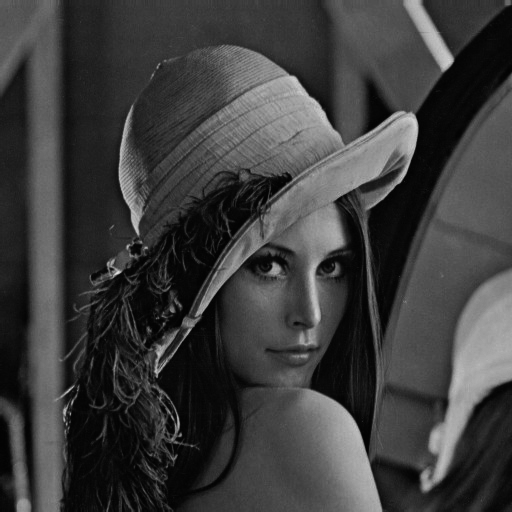
\includegraphics[width=0.50\textwidth]{img/grey.png}
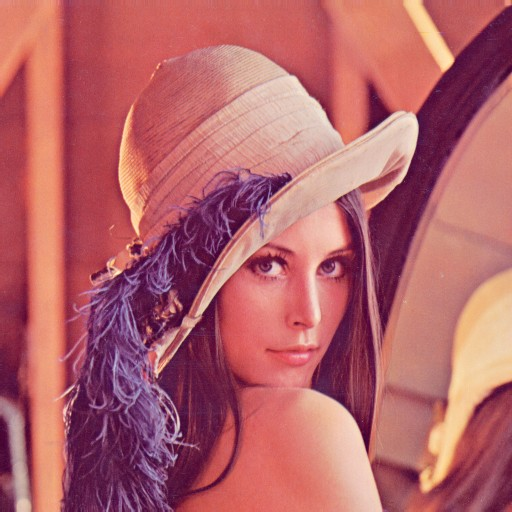
\includegraphics[width=0.50\textwidth]{img/lena.jpg}
\caption{avec et sans nuance (captain obvious is obvious)}
\end{figure}
\newpage{}
\subsubsection{Le filtre median}
\subsubsubsection{\textbf{Le concept}}:\\
Le filtre median va pour chaque pixels de l'image recupere le triplet (R,G,B) de chaque pixel autour du pixel traite et trier ces pixels par ordre croissant. Il suffit juste de recuperer la valeur mediane de la liste trier. Le passe dans cette algo et qyue l'on doit passer les pixels sur une autre image pour pas fausser les calculs sur la premiere image !
\subsubsubsection{\textbf{La realisation}}\\
En pratique ce filtre ne s'applique pas sur toute les images car sinon elle floute l'image et la rend intraitable. Je suis actuellement en recherche d'un algorithme permettant de palier ce gros probleme. Au niveau aulgoritemiaue on obtiens
\begin{figure}[h]
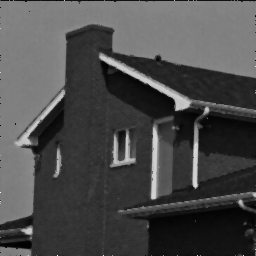
\includegraphics[width=0.50\textwidth]{img/house.png}
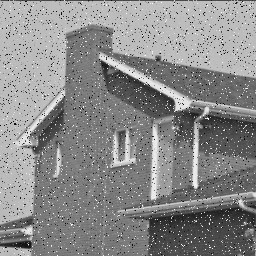
\includegraphics[width=0.50\textwidth]{img/house.jpg}
\caption{presentation du filtre median}
\end{figure}
\subsubsection{La binarisation}
\subsubsubsection{\textbef{Le concept}}:\\
Nous utilisons l'algorithme d'Otsu, du nom de son inventeur Nobuyuki Otsu. Qui se base sur l'histogramme d'un image. L'histogramme est un tableau de 255 element, ici des entiers, qui represente le nombre d'occurence d'un niveau de gris ( les niveau de gris allant de 0 (blanc) a 255 (noir). Dans un permier temps va creer un tableau pour y mettre les valeur traiter de l'histogramme de la maniere suivant 
\begin{center}
\[ p_{i} = \frac{h_{i}} {width * height}\]
\end{center}
qui renvoie la population du niveau de gris i dans l'ensemble des pixels de l'image.
\subsubsection{Détection d'angle}
Je me suis donc occupe de la transformation de Hough. La transforme de hough est une techmiaue de reconnaissance de formes invente en 1962 par Paul Hough.
Le principe qui sous-tend la transforme de Hough est qu'il existe un nombre infini de ligne passant par un point dont la seule difference est l'orientation (l'angle). La transforme generalise de Houg fonctionne sur le principe qu'une droite peux s'ecrire sous la forme 
\[r = x\cos{\theta}+y\sin{\theta}\]
A chaque pixels noir on essaye de trouver la vlauer maximum de r. Cette valeur represente la droite qui alligne le plus de pixel noir. On la retiens et on vote dans un tableau pour son angle associer. On recommence sur tout les pixels. L'angle qui a recu le plus de vote estl'anlge de rotation de l'image( minore de la moitier de l'intervalle pour pouvoir faire ressortir les angles negatifs).
\\
Voici le principe de l'algo en pseudo code :
\begin{lstlisting}
for y =0 to hauteur de l'image do
    for x =0 to largeur de l'image do
        if (pixel noir ) then
           angle = -Pi/2
           while (angle < Pi/2) do
            begin
              r = x*cos(angle)+y*sin(angle)
              if(r>o) then
             /* increment tableau de vote */          
              angle ++
            end
        end
     done
done

\end{lstlisting} 

\begin{figure}[hp]
\centering
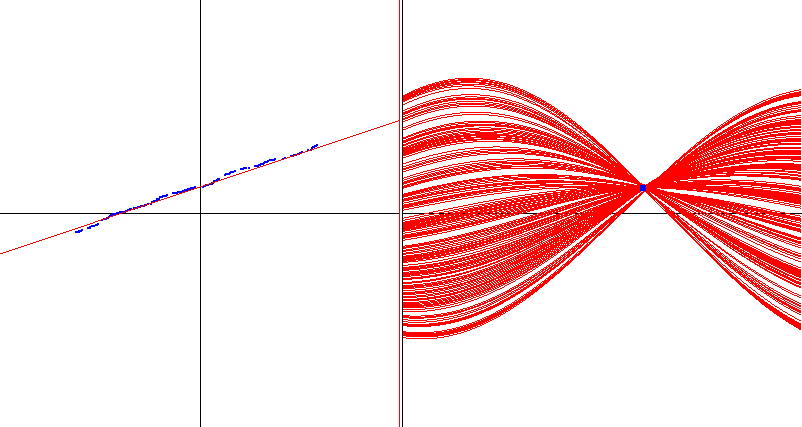
\includegraphics[width=0.80\textwidth]{img/hough.png}
\end{figure}
\subsection{La rotation}
La rotation est effectue grace a une matrice de rotation. La methode consiste a assosicie chaque pixel (i, j) a une matrice [|[|i|]; [|j|]|] puis d'utilliser la formule suivate : 
$A_{i,j}R_{\theta} = A'_{i,j}$ avec R = [|[|cos \theta; -sin \theta|]; [|sin \theta; cos \theta|]|] 
Le resultat sera alors de la forme [|[|i'|]; [|j'|]|], il faut alors creer une image d'une (diag, diag) avec diag la diagonal de l'image source, puis assigne la couleur du pixel (i, j) au pixel (i', j').

\subsection{Decoupage de l'image}
\subsection{Perceptron}
Un perceptron est compose dune liste de poids, grace a un certain nombre d'entre et a une fonction dite a seuil, il va fournir une sortie grace a la formule suivante: 
$\sigma entree_{i}.poids_{i} > seuil$
 La sortie sera 1 si l'equation est verifie, 0 sinon. Par exemple un perceptron qui peut analyser une porte OU repondra a l'entree (0, 1) par 1.
Une fois le perceptrion structure il faut quil puisse apprendre, cest a dire modifier ses poids pour qu'il donne de bons resultas. Pour ce faire il faut lui passer une batterie de tests avec les resultats escomptes. On va alors evaluer le neurone avec un test et regarder si le resultat est le bon, si ce n'est pas le cas le poid va alors etre corrige selon la formule suivante: 
$poid = poid + entree*(sortieVoulu - sortieReel)$.
 Ces tests sont effectues jusqu'a ce que toutes les sorties soient bonnes: le perceptron a alors appris.


\subsection{Réseau de neurone}
Un neurone est tres semblant a un perceptron, au fait pret que sa sortie n'est pas binaire: il n'utilise pas une fonction a seuil mais une fonction sigmoide de la forme: 
$f(x) = 1 / 1 + \exp ^{k.-x}$
Un reseau de neurone est compose de n couche de neurone, une couche de neurone est compose de m neurone, chaque neurone est relie avec tout les neurones de la couche precedente. Un reseau de neurone prend une liste d'entree et va fournir une liste de sortie.

\section{Conclusion}


\end{document}
